\chapter{Anwendungen}

Die zuvor in Kapitel \ref{ch:theory} eingeführten Methoden werden nun durch drei verschiedene Szenarien ausprobiert und verglichen. Hierbei liegt der Fokus auf der Verwendung und Erprobung der \textsc{ESN}s. Da die klassischen Methoden der \textit{nächsten Nachbarn} und der \textit{radialen Basisfunktionen} bereits seit längerer Zeit bekannt sind und populäre Lösung solcher Problemfälle darstellen, dienen sie als Bezugsgröße.\\

Jedes der drei Szenarien wird sowohl auf ein \textit{Barkley}-System als auch auf ein System nach dem \textit{Mitchell-Schaeffer}-Modell angewendet. Diese Systeme bestehen aus $150$ Gitterpunkten und nutzen die zuvor beschriebenen Parameter. Für ihre Startverteilung werden die Felder der beiden Systemvariablen in $100$ Quadrate unterteilt, und diese mit Zufallswerten zwischen $0$ und $1$ initialisiert. Anschließend werden die Systeme über $2000$ Zeitschritte ($\widehat{=} 400.0$ Zeiteinheiten) simuliert um ein transientes Verhalten abzuwarten. Durch das weitere Simulieren der Systeme werden die Test und Trainingsdaten ermittelt. Dabei wird für das \textit{Barkley} eine Samplingzeit von $0.1$ und für das \textit{Mitchell-Schaeffer}-Modell von $1.0$ Zeiteinheiten benutzt.\\
 
Die erste Aufgabe besteht darin aus der Kenntnis einer der beiden Systemvariablen die andere Unbekannte zu ermitteln. Dabei wird die Spannungsvariable als Quelle genutzt. Dies ist in den zuvor eingeführten Modellen jeweils die Größe, welche den Diffusionsterm beinhaltet; also die $u$-Variable im \textit{Barkley}-Modell und die $v$-Variable im \textit{Mitchell-Schaeffer}-Modell.\\
Im zweiten Szenario werden die Techniken verwendet um aus Messdaten einer simulierten Fernfeldmessung der Spannungsvariable  diese wiederherzustellen. Diese Fernfeldmessung wird durch eine gaußsche Unschärfe simuliert.\\
Abschließend wird die Spannungsvariable der inneren Punkte eines Quadrates nur durch die Kenntnis der Randwerte des Systems vorhergesagt.\\

%TODO ADD SUBCHAPTER?
\section{Allgemeines Vorgehen}
\label{sc:experiments_general}
Das Ziel aller drei Aufgaben besteht jeweils darin ein zweidimensionales Feld vorherzusagen. Eine naheliegende Möglichkeit dies zu schaffen besteht darin wirklich den gesamten Inhalt des $150 \times 150$ Einheiten großen Feldes auf einmal vorherzusagen. Da dabei die Ausgabe der Vorhersage aus einem $22500$-dimensionalen Vektor besteht werden sehr viele Trainingsdaten benötigt, um genügend Informationen über eine solch hochdimensionale Ausgabe zu erhalten. Um dieses Problem zu umgehen wird stattdessen ein Verfahren benutzt, bei dem jeder Punkt einzeln vorhergesagt wird. Dies hat zudem den Vorteil, dass aus einer monströsen Vorhersage, welche mitunter viel Arbeitsspeicher verbrauchen würde, in viele kleine Vorhersagen aufteilt. Hierdurch sinkt der zur Berechnung benötigte Bedarf an Arbeitsspeicher drastisch.\\

Des Weiteren kann angenommen werden, dass die Dynamiken einen ausgeprägten lokalen Charakter besitzen, sodass zumindest bei den ersten beiden Aufgaben weit entfernte Punkte keinen unmittelbaren Einfluss auf die Vorhersage haben. Darauf basierend kann eine sogenannte \textit{Messsondentechnik} entwickelt und genutzt werden. Hierbei werden nicht nur die Informationen an einem Punkt $(i, j)$ für die Vorhersage, sondern auch die benachbarten Punkte, welche in einem Quadrat um $(i, j)$ liegen, genutzt. Eine Veranschaulichung ist in \ref{fig:probe_illustration_no_gaps} zu finden. Die Größe des Quadrates wird durch den Parameter $\sigma$ bestimmt, und ergibt sich zu $\sigma^2$. Da direkt Nachbarn unter Umständen durch den geringen Abstand sehr ähnliche Informationen beinhalten können, wird zudem ein Parameter $\Delta \sigma$ eingeführt, welche den Abstand zweier benachbarter Punkte, deren Information simultan verwendet werden, angibt. Eine beispielhafte Darstellung hiervon ist für $\sigma = 5, \Delta \sigma=2$ in Abbildung \ref{fig:probe_illustration_gaps} dargestellt. Dabei werden nur die Zeitreihen der Gitterpunkte genutzt, welche dunkelgrau hinterlegt sind, und die hellgrauen Informationen verworfen.\\
Durch dieses Vorgehen kann für jeden Gitterpunkt ein ${\left \lceil{\frac{\sigma}{\Delta \sigma}}\right \rceil}^2$-dimensionaler Eingabevektor erstellt und für die ersten beiden Vorhersage-Aufgaben genutzt werden.

\begin{figure}[h]
\centering
\begin{subfigure}{.5\textwidth}
  \centering
  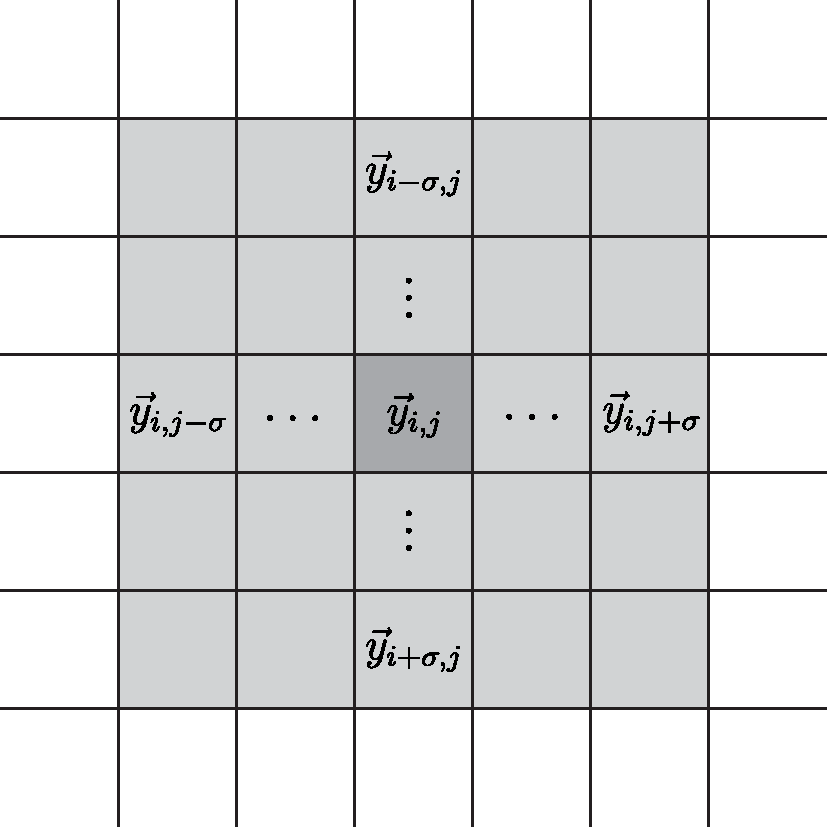
\includegraphics[width=.8\linewidth]{figures/illustrations/sigma_patches.pdf}
  \caption{Messsonde ohne Abstände zwischen\\den Messpunkten}
  \label{fig:probe_illustration_no_gaps}
\end{subfigure}%
\begin{subfigure}{.5\textwidth}
  \centering
  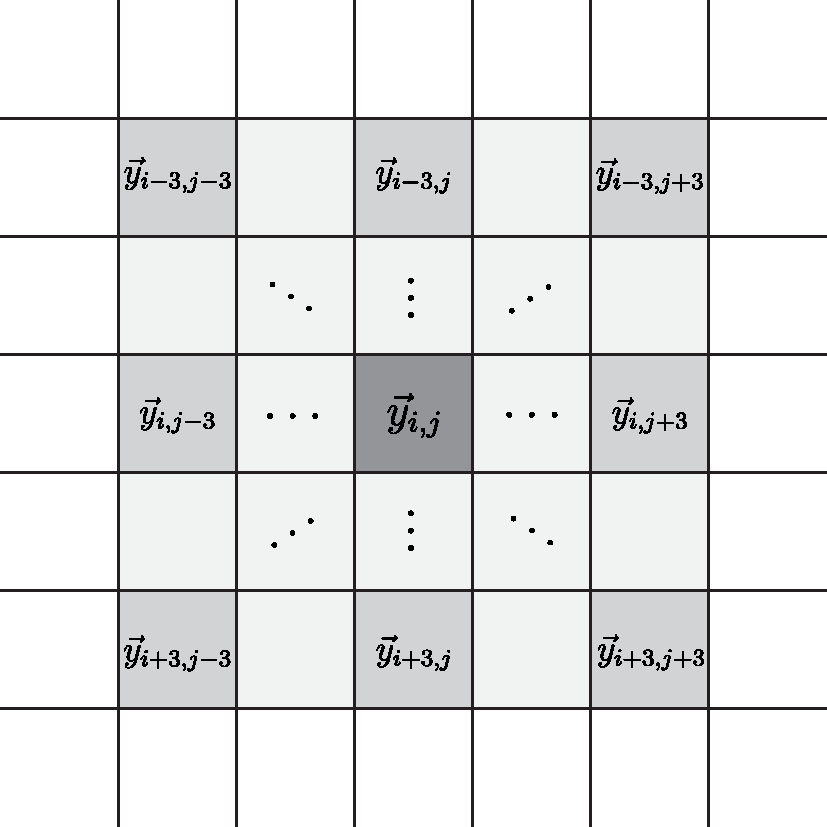
\includegraphics[width=.8\linewidth]{figures/illustrations/sigma_patches_gaps.pdf}
  \caption{Messonde mit einem Abstand von zwei Einheiten zwischen den Messpunkten}
  \label{fig:probe_illustration_gaps}
\end{subfigure}
\caption{Illustration der verwendeten \textit{Messsondentechnik}. Abbildung \ref{fig:probe_illustration_no_gaps} deutet an, wie aus einem $\sigma^2$ großem Quadrat um den eigentlichen Messpunkt Daten für die Vorhersage genutzt werden. Dagegen ist in Abbildung \ref{fig:probe_illustration_gaps} das Verfahren für $\sigma=5$ und $\Delta \sigma = 2$ dargestellt, sodass insgesamt die Information aus $9$ Punkten genutzt wird.}
\label{fig:probe_illustration}
\end{figure}

\subsection{Echo State Network}
\textit{Echo State Networks} besitzen viele verschiedene Hyperparameter, welche die Qualität der Vorhersage beeinflussen können. Dazu zählen nach \ref{sc:esn} die Reservoirgröße $N$, der Spektralradius $\rho$, die Verlustrate $\alpha$, die Amplitude der zufälligen Störung $\nu$, die Stärke der Regularisierung $\lambda$ und der Anteil der vorhandenen internen Verbindungen $\epsilon$. Da es zum aktuellen Zeitpunkt noch keinen zufriendenstellenden mathematischen Algorithmus für das das selbstständige optimale Einstellen eines \textsc{ESN}s gibt, müssen die Parameter manuell ermittelt werden. Hierfür wird in dieser Arbeit eine \textsc{GridSearch} benutzt. Bei diesem Verfahren wird der Hyperparameterraum in festgelegten Schritten abgetastet und die Leistung des somit entstehenden Netzwerke evaluiert und somit die besten Parameter ermittelt. Durch die hohe Anzahl der einstellbaren Hyperparameter und die nicht zu vernachlässigende Rechenzeit für das Trainieren und Evaluieren eines Netzwerkes, ist es nicht sinnvoll diese Suche für alle Datenpunkte gleichzeitig durchzuführen. Stattdessen wird zuerst unter der Annahme, dass die Dynamik sich lokal an allen Punkten ähnlich verhält, ein Punkt in der Mitte des Feldes ausgewählt, und nur versucht dieses einen einzelnen Punkt vorherzusagen. Diese Aufgabe kann deutlich schneller berechnet werden, sodass nun die optimalen Hyperparameter mit einer \textsc{GridSearch} gesucht werden können. Anschließend können die Hyperparameter des  zuvor ermittelten \textsc{ESN} für die Vorhersage aller Punkte genutzt werden.

\subsection{Klassische Methoden}
Die klassischen Methoden sind nicht von alleine aus in der Lage zeitlich ausgeprägte Dynamiken vorherzusagen, da den Methoden a priori keine Informationen über die vorherigen Zustände vorliegen. Um dieses Problem zu lösen können Verzögerungs-Koordinaten mittels der in Abschnitt \ref{sc:delay_reconstruction} beschriebenen \textit{Delay Reconstruction} für die in Abschnitt \ref{sc:experiments_general} beschriebenen Vektoren aufgestellt werden. Die über die Autokorrelation ermittelte zeitliche Verzögerung $\tau$ ist für beide Systeme in Tabelle \ref{tab:delay_reconstruction_tau} dargestellt.     

\begin{table}[h]
\centering
\begin{tabular}{|c|c|}
$\tau_{Barkley}$ & $\tau_{Mitchell-Schaeffer}$ \\ 
\hline 
\hline 
0.64 Zeiteinheiten & 2.38 Zeiteinheiten\\ 
\hline 
\end{tabular} 
\caption{Verwendete zeitliche Verzögerung $\tau$ für die \textit{Delay Reconstruction} für das \textit{Mitchell-Schaeffer}- und das \textit{Barkley}-Modell}
\label{tab:delay_reconstruction_tau}
\end{table} 

\section{Kreuz-Prädiktion}
\label{sec:exp_cross_pred}
Momentan ist es durch invitro Experimente bereits möglich die Ausbreitung der elektrischen Erregung auf der Oberfläche des Herzmuskels experimentell aufzuzeichnen. Nun stellt sich die Frage, ob anhand beispielsweise der Messung der Membramspannung weitere Variablen des Systems wie die Kalium-Konzentration oder ähnliches ermittelt werden kann. Diese Fragestellung wird in der ersten Aufgabe betrachtet. Es wird die Vorhersage von der Spannungsvariable auf die zweite Variable des jeweiligen Modells sowohl für das \textit{Barkley}- als auch für das \textit{Mitchell-Schaeffer}-Modell durchgeführt. Dabei wird zuerst die Nächste Nachbar Methode, anschließend die radialen Basisfunktionen und schlussendlich die \textit{ESN}s verwendet. Es werden sowohl die einzelnen Ergebnisse präsentiert als auch ein abschließender Vergleich durchgeführt.
 
\subsection{Nächste Nachbar Vorhersage}
Die Ergebnisse für die optimalen Hyperparameter sind in Tabelle \ref{tab:exp_cross_nn_results} zu finden. Dabei sind sowohl die verwendeten Parameter als auch die erzielten Fehler MSE und NRMSE aufgelistet.
\begin{table}[h]
	\centering

	\begin{tabular}{|c|c|c|}
		\multicolumn{1}{c|}{} & Barkley & Mitchell-Schaeffer \\ 
		\hline \hline 
		\rule[-1ex]{0pt}{2.5ex} $\sigma$ & $1$ & $7$ \\ 
		\hline 
		\rule[-1ex]{0pt}{2.5ex} $\Delta \sigma$ & $1$ & $1$ \\ 
		\hline 
		\rule[-1ex]{0pt}{2.5ex} $\delta$ & $3$ & $3$ \\ 
		\hline 
		\rule[-1ex]{0pt}{2.5ex} k & $5$ & $5$ \\ 
		\hline 
		\rule[-1ex]{0pt}{2.5ex} Laufzeit [s] & $40$ & $5252$ \\ 
		\hline 
		\rule[-1ex]{0pt}{2.5ex} \textbf{MSE} & \textbf{0.00105} & \textbf{0.01353} \\ 
		\hline 
		\rule[-1ex]{0pt}{2.5ex} \textbf{NRMSE} & \textbf{0.1367} & \textbf{0.7438} \\ 
		\hline 
	\end{tabular} 

	\caption{Gefundene Hyperparameter der nächsten Nachbar Vorhersage für das \textit{Mitchell-Schaeffer}- und das \textit{Barkley}-Modell, welche zu den geringsten Fehlern führen.}
\label{tab:exp_cross_nn_results}
\end{table} 

Dabei ist die stark unterschiedliche Laufzeit der beiden Vorhersagen auffällig. Dies lässt sich allerdings durch die verschiedenen Dimensionalitäten der Quellvariable erklären: Während beim \textit{Barkley}-Modell lediglich ein $3$-dimensionaler Vektor für die Vorhersage die besten Ergebnisse erzielt konnte beim \textit{Mitchell-Schaeffer}-Modell durch die Verwendung eines $147$-dimensionalen Quellvektors die besten Ergebnisse erzielt werden. Da, wie in Abschnitt \ref{sc:theory_nn} erwähnt, die benötigte Zeit für eine Vorhersage sehr stark mit der Dimension zunimmt, lässt sich somit der Anstieg von $40$ auf $5252$ Sekunden erklären.

Da eine Nächsten Nachbar Vorhersage nur anhand der in der Trainingsphase gesehenen Datenpunkte eine Vorhersage erstellt, ist anzunehmen, dass die Qualität dieser sehr stark von der Länge der Trainingsphase abhängt. Um dies zu untersuchen ist für die zuvor ermittelten Hyperparameter eine Vorhersage für verschiedene Trainingslängen $N_{Training}$ durchgeführt und die dabei auftretenden MSEs und die benötigte Laufzeit gemessen worden. Hierbei können zwei Effekte beobachtet werden. Bei der Betrachtung der grafischen Darstellung der benötigten Laufzeit in Abbildung \ref{fig:exp_cross_nn_trainlength_time} ist zu erkennen, dass ein linearer Zusammenhang zwischen der $N_{Training}$ und Laufzeit existiert. Der erzielte Fehler verhält sich dagegen anders und sinkt asymptotisch gegen eine untere Schranke ab nach Abbildung \ref{fig:exp_cross_nn_trainlength_mse}. Anzumerken ist, dass die Sättigung des Fehlers im \textit{Barkley}-Modell schon ab etwa $N_{Training}=15000$ eintritt, doch beim \textit{Mitchell-Schaeffer}-Modell erst deutlich später. Dies ist ein Hinweis darauf, dass die Dynamiken im letzteren chaotischer und unregelmäßiger als bei ersten ablaufen. Zusammenfassend lässt sich somit die Wahl der Trainingslänge von $N_{Training} = 15000$ für alle Szenarien und alle drei Methoden damit begründen, dass man für die Nächste Nachbar Vorhersage, welche am empfindlichsten auf diese Länge reagiert, eine akzeptablen Kompromiss zwischen der Rechenzeit und der Genauigkeit erhält.

\begin{figure}[h]
	\centering
	\begin{subfigure}{.5\textwidth}
		\centering
		\includegraphics[height=2.2in]{figures/results/cross_prediction/nn_trainlength_uv_time.pdf}
		\setcapmargin[1cm]{1cm}
		\caption{Abhängigkeit für das \\ \textit{Barkey}-Model.}
		\label{fig:exp_cross_nn_trainlength_time_uv}
	\end{subfigure}%
	\begin{subfigure}{.5\textwidth}
		\centering
		\includegraphics[height=2.2in]{figures/results/cross_prediction/nn_trainlength_vh_time.pdf}
		\setcapmargin[1cm]{1cm}
		\caption{Abhängigkeit für das \\ \textit{Mitchell-Schaeffer}-Model.}
		\label{fig:exp_cross_nn_trainlength_time_vh}
	\end{subfigure}
	\caption{Darstellung der Abhängigkeit des benötigten Laufzeit von der verwendeten Anzahl an Trainingsdaten $N_{Training}$ für das \textit{Barkley}-Modell (links) und für das \textit{Mitchell-Schaeffer}-Modell (rechts) bei der Verwendung einer nächsten Nachbar Vorhersage.}
	\label{fig:exp_cross_nn_trainlength_time}
\end{figure}

\begin{figure}[h]
	\centering
	\begin{subfigure}{.5\textwidth}
		\centering
		\includegraphics[height=2.2in]{figures/results/cross_prediction/nn_trainlength_uv_mse.pdf}
		\setcapmargin[1cm]{1cm}
		\caption{Abhängigkeit für das \\ \textit{Barkey}-Model.}
		\label{fig:exp_cross_nn_trainlength_mse_uv}
	\end{subfigure}%
	\begin{subfigure}{.5\textwidth}
		\centering
		\includegraphics[height=2.2in]{figures/results/cross_prediction/nn_trainlength_vh_mse.pdf}
		\setcapmargin[1cm]{1cm}
		\caption{Abhängigkeit für das \\ \textit{Mitchell-Schaeffer}-Model.}
		\label{fig:exp_cross_nn_trainlength_mse_vh}
	\end{subfigure}
	\caption{Darstellung der Abhängigkeit des MSE von der verwendeten Anzahl an Trainingsdaten $N_{Training}$ für das \textit{Barkley}-Modell (links) und für das \textit{Mitchell-Schaeffer}-Modell (rechts) bei der Verwendung einer nächsten Nachbar Vorhersage.}
	\label{fig:exp_cross_nn_trainlength_mse}
\end{figure}

\FloatBarrier
\subsection{Radiale Basisfunktionen}
Bei der Verwendung radialer Basisfunktionen stellt zudem die Breite $\sigma_{RBF}$ der Gaußfunktionen als auch die Anzahl der Basisfunktionen $l$ einen wichtigen Parameter dar. Im Rahmen dieser Arbeit ist die Anzahl der Basisfunktionen auf $l=100$ festgelegt worden - diese Wahl wird im Folgenden weiter motiviert werden. Um die anderen Parameter zu finden, sind $\sigma$, $\Delta \sigma$ wie oben beschrieben, $\delta \in [3,4,5]$ und $\sigma_{RBF} \in [0.5, 1.0, 3.0, 5.0, 7.0, 9.0]$ variiert worden. In Tabelle \ref{tab:exp_cross_rbf_results} sind die dadurch gefundenen optimalen Parameter, die damit erreichten Fehler und die benötigte Laufzeit erneut für beide Modelle aufgelistet. Hierbei ist zu bemerken, dass die optimalen Werte für $\sigma$, $\Delta \sigma$ und $\delta$ mit denen für die NN-Vorhersage übereinstimmen. 

\begin{table}[h]
	\centering

	\begin{tabular}{|c|c|c|}
		\multicolumn{1}{c|}{} & Barkley & Mitchell-Schaeffer \\ 
		\hline \hline 
		\rule[-1ex]{0pt}{2.5ex} $\sigma$ & $1$ & $7$ \\ 
		\hline 
		\rule[-1ex]{0pt}{2.5ex} $\Delta \sigma$ & $1$ & $1$ \\ 
		\hline 
		\rule[-1ex]{0pt}{2.5ex} $\delta$ & $3$ & $3$ \\ 
		\hline 
		\rule[-1ex]{0pt}{2.5ex} $\sigma_{RBF}$ & $0.5$ & $5$ \\ 
		\hline 
		\rule[-1ex]{0pt}{2.5ex} Laufzeit [s] & $1430$ & $1434$ \\ 
		\hline 
		\rule[-1ex]{0pt}{2.5ex} \textbf{MSE} & \textbf{0.00064} & \textbf{0.00890} \\ 
		\hline 
		\rule[-1ex]{0pt}{2.5ex} \textbf{NRMSE} & \textbf{0.1069} & \textbf{0.6034} \\ 
		\hline 
	\end{tabular} 
	\caption{Gefundene Hyperparameter der radialen Basisfunktionen für das \textit{Mitchell-Schaeffer}- und das \textit{Barkley}-Modell, welche zu den geringsten Fehlern führen.}
	\label{tab:exp_cross_rbf_results}
\end{table} 

Analog zu der Untersuchung des Einflusses der Trainingslänge $N_{Training}$ bietet es sich für die radialen Basisfunktionen an, den Einfluss der Anzahl der verwendeten Basisfunktionen $l$ auf die Genauigkeit und die benötigte Laufzeit zu untersuchen. Dabei werden jeweils wieder die besten zuvor ermittelten Hyperparameter verwendet. Hierfür sind die gemessenen Laufzeiten gegen die Anzahl der Basisfunktionen in Abbildung \ref{fig:exp_cross_rbf_placements_time} aufgetragen worden. Es ist erneut anzunehmen, dass ein linearer Zusammenhang zwischen den beiden Größen existiert.

\begin{figure}[h]
	\centering
	\begin{subfigure}{.5\textwidth}
		\centering
		\includegraphics[height=2.2in]{figures/results/cross_prediction/rbf_placements_uv_time.pdf}
		\setcapmargin[1cm]{1cm}
		\caption{Abhängigkeit für das \textit{Barkey}-Model.}
		\label{fig:exp_cross_rbf_placements_time_uv}
	\end{subfigure}%
	\begin{subfigure}{.5\textwidth}
		\centering
		\includegraphics[height=2.2in]{figures/results/cross_prediction/rbf_placements_vh_time.pdf}
		\setcapmargin[1cm]{1cm}
		\caption{Abhängigkeit für das \textit{Mitchell-Schaeffer}-Model.}
		\label{fig:exp_cross_rbf_placements_time_vh}
	\end{subfigure}
	\caption{Darstellung der Abhängigkeit des benötigten Laufzeit der Basisfunktionen $l$ für das \textit{Barkley}-Modell (links) und für das \textit{Mitchell-Schaeffer}-Modell (rechts) bei der Verwendung radialer Basisfunktionen.}
	\label{fig:exp_cross_rbf_placements_time}
\end{figure}

Der Zusammenhang zwischen dem MSE und der Anzahl der Basisfunktionen ist in Abbildung \ref{fig:exp_cross_rbf_placements_mse} zusehen. Zum einen kann ein ein asymptotischer Anteil erkannt werden, sodass der Fehler erst einmal für mehr Basisfunktionen abnimmt. Allerdings lässt Abbildung \ref{fig:exp_cross_rbf_placements_mse_uv} erahnen, dass es hierbei einen optimalen Wert gibt, ab dem der Fehler wieder ansteigt. Dies kann durch eine schlechtere Generalisierung der Dynamik und ein zu starkes Anpassen und die Trainingsphase (auch bekannt als \textit{Overfitting}) erklärt werden. Zusammenfassend zeigt sich, dass die Wahl von $100$ Basisfunktionen eine akzeptable Abschätzung ist, sodass der Fehler möglichst gering ist und die Laufzeit auch gering gehalten wird. Diese Annahme wird im Folgenden ohne weitere qualitative Untersuchungen auf die anderen beiden Probleme übertragen, um den benötigten Rechenaufwand für die Parametersuche in einem angebrachten Rahmen zu halten.  

\begin{figure}[h]
	\centering
	\begin{subfigure}{.5\textwidth}
		\centering
		\includegraphics[height=2.2in]{figures/results/cross_prediction/rbf_placements_uv_mse.pdf}
		\setcapmargin[1cm]{1cm}
		\caption{Abhängigkeit für das \textit{Barkey}-Model.}
		\label{fig:exp_cross_rbf_placements_mse_uv}
	\end{subfigure}%
	\begin{subfigure}{.5\textwidth}
		\centering
		\includegraphics[height=2.2in]{figures/results/cross_prediction/rbf_placements_vh_mse.pdf}
		\setcapmargin[1cm]{1cm}
  		\caption{Abhängigkeit für das \textit{Mitchell-Schaeffer}-Model.}
  		\label{fig:exp_cross_rbf_placements_mse_vh}
	\end{subfigure}
	\caption{Darstellung der Abhängigkeit des MSE von der verwendeten Anzahl der Basisfunktionen $l$ für das \textit{Barkley}-Modell (links) und für das \textit{Mitchell-Schaeffer}-Modell (rechts) bei der Verwendung radialer Basisfunktionen.}
	\label{fig:exp_cross_rbf_placements_mse}
\end{figure}

\FloatBarrier
\subsection{Echo State Network}
Abschließend ist dieses Problem nun mit den \textit{ESN}s gelöst worden. Dazu wurden die Hyperparameter nach Abschnitt \ref{sec:exp_general_esn} gesucht worden. Die gefundenen Parameter und die damit erreichten Ergebnisse sind in Tabelle \ref{tab:exp_cross_esn_results} aufgelistet. Es ist auffällig, dass die optimalen Werte für $\sigma$ und $\Delta \sigma$ hier von denen der NN- und der RBF-Vorhersage abweichen.
\begin{table}[h]
	\centering
	\captionsetup{width=0.9\linewidth}
	\begin{tabular}{|c|c|c|}
		\multicolumn{1}{c|}{} &  Barkley & Mitchell-Schaeffer \\ 
		\hline \hline 
		\rule[-1ex]{0pt}{2.5ex} $\sigma$ & $3$ & $3$ \\ 
		\hline 
		\rule[-1ex]{0pt}{2.5ex} $\Delta \sigma$ & $1$ & $1$ \\ 
		\hline 
		\rule[-1ex]{0pt}{3.5ex} $N$ & $400$ & $400$ \\ 
		\hline 
		\rule[-1ex]{0pt}{3.5ex} $\rho(|\mathbf{W}|)$ & $0.95$ & $0.95$\\ 
		\hline 
		\rule[-1ex]{0pt}{3.5ex} $\alpha$ & $0.05$ & $0.05$ \\ 
		\hline 
		\rule[-1ex]{0pt}{3.5ex} $\epsilon$ & $0.1$ & $0.1$ \\ 
		\hline 
		\rule[-1ex]{0pt}{3.5ex} $\nu_{max}$ & $\num{1e-4}$ & $\num{1e-4}$\\ 
		\hline 
		\rule[-1ex]{0pt}{3.5ex} $\lambda$ & $\num{5e-6}$ & $\num{5e-6}$\\ 
		\hline 
		\rule[-1ex]{0pt}{2.5ex} Laufzeit [s] & $3710$ & $3733$ \\ 
		\hline 
		\rule[-1ex]{0pt}{2.5ex} \textbf{MSE} & \textbf{\num{1.95e-7}} & \textbf{0.00075} \\ 
		\hline
		\rule[-1ex]{0pt}{2.5ex} \textbf{NRMSE} & \textbf{\num{3.47e-6}} & \textbf{0.1753} \\ 
		\hline 
	\end{tabular} 
	\caption{Gefundene Hyperparameter des \textsc{ESN} für das \textit{Mitchell-Schaeffer}- und das \textit{Barkley}-Modell, welche zu den geringsten Fehlern führen.}
	\label{tab:exp_cross_esn_results}
\end{table}

Auffällig ist, dass für beide Modelle die gleichen Hyperparameter die höchste Genauigkeit erzielen. 
\improvement{Add more details?}

\FloatBarrier
\subsection{Vergleich}
Abschließend kann nun ein Vergleich der drei verwendeten Methoden hinsichtlich ihrer Laufzeit und der erzielten Genauigkeiten durchgeführt werden. Dieser ist in Tabelle \ref{tab:exp_cross_comparison_results} zu finden. Die jeweils  besten Ergebnisse sind hervorgehoben. Die \textit{ESN}s erzielen für beide Modelle den geringsten Fehler, also die höchste Genauigkeit. Dabei ist der NRMSE für das \textit{Barkley}-Modell mehrere Größenordnung kleiner als bei den Konkurrenz-Ansätzen. Diese überaus hohe Genauigkeit ist für das \textit{Mitchell-Schaeffer}-Modell nicht erreicht worden. Hier beträgt der Fehler trotzdem etwa nur ein Drittel von dem der anderen Ansätze. Im Austausch für diese hohe Genauigkeit ist allerdings die benötigte Zeit für die Vorhersage höher als bei den Konkurrenten. Unter der Voraussetzung, dass die Rechenzeit nur eine untergeordnete Rolle spielt, so ergeben sich die \textit{ESN}s als bester Ansätze für die Kreuz-Prädiktion.
\begin{table}[h]
	\centering
	\captionsetup{width=0.9\linewidth}
	\begin{tabular}{|c|c|c|c|c|c|c|c|}
		\multicolumn{1}{c|}{} & \multicolumn{3}{c|}{Barkley} & \multicolumn{3}{c|}{Mitchell-Schaeffer}		\\
		\cline{2-7}
		\multicolumn{1}{c|}{} & NN & RBF & ESN & NN & RBF & ESN \\
		
		\hline
		\hline
		
		Laufzeit [s] 	& \textbf{40} 		& 1430		& 3710		& 5252		& \textbf{1434} 		& 3733 \\
		\hline
		MSE 			& 0.00105	& 0.00064	& \textbf{\num{1.95e-7}} 	& 0.01353	& 0.00890 	& \textbf{0.00075} \\
		\hline
		NRMSE 			& 0.1367	& 0.1069	& \textbf{\num{3.47e-6}} 	& 0.7438	& 0.6034 	& \textbf{0.1753} \\
		\hline 
	\end{tabular} 
	\caption{Vergleich der benötigten Laufzeit und der erreichten Fehlers der drei Ansätze für das \textit{Mitchell-Schaeffer}- und das \textit{Barkley}-Modell, welche zu den geringsten Fehlern führen.}
	\label{tab:exp_cross_comparison_results}
\end{table}

\FloatBarrier
\section{Kreuz-Prädiktion innere Dynamiken}
Bei Messungen der elektrischen Erregung des Herzens können nach aktuellen Stand meistens nur die Erregungen auf der Herzoberfläche gemessen werden. Die Ausbreitungen im Inneren des räumlich ausgedehnten Herzens bleiben somit verborgen. Zudem ist anzunehmen, dass die Gesamtdynamik nicht nur durch die Oberfläche, sondern auch durch die Erregung im Inneren bestimmt und charakterisiert wird. Somit wird die Frage aufgeworfen, ob die innere Erregung des Herzens nur durch die Kenntnis der Oberflächendynamik vorhergesagt werden kann. In diesem Abschnitt soll versucht werden, diese Fragestellung erneut mit den \textsc{ESN}s und den klassischen Methoden zu untersuchen. Dabei wird statt eines dreidimensionalen Systems diese Frage an den zuvor bereits benutzten zweidimensionalen Modellen betrachtet.\\
\section{Prädiktion der Dynamik durch das Fernfeld}